\section{Preliminaries}\label{Section:Preliminaries}
%Need for handling uncertainty in data streams.
%BNs as the natural solution.

The following sections aim at describing some of the concepts and basic structures required to easily interpret the AMIDST models that will be proposed for the different use cases below. Section \ref{SubSection:HybridBNs} briefly introduces the challenges encountered for reasoning with continuous and discrete variables. Section \ref{SubSection:DBNs} describes some of the basic concepts and models related to dynamic Bayesian reasoning over time. Section \ref{SubSection:DataAnalysis} defines the data analysis techniques used to support many of the assumptions made on the proposed models.


\subsection{Static Hybrid Bayesian networks}\label{SubSection:HybridBNs}
%Talk about the challenges of discrete children with continouous parents.
Traditionally, Bayesian networks have been defined for discrete domains, where the entities of interest are modelled by discrete variables which ensures that belief updating can be performed efficiently and in closed form. However, this requirement also imposes severe restrictions as many domains contain entities that are more appropriately modelled by variables with continuous state spaces; an example is distance and velocity measurements, which are key sensor readings for identifying and interpreting manoeuvres in traffic (see Daimler's requirement analysis \cite{Fer14}). To extend probabilistic graphical models with support for continuous variables research has largely pursued three directions. Firstly, one may choose to carefully construct the model such that exact inference algorithms can still be applied. This is the case for the linear Gaussian (CLG) Bayesian networks \cite{Lauritzen1992,LauritzenJensen2001}, where the local probability distributions of the continuous variables are specified as conditional linear Gaussian distributions and discrete variables can only have discrete parents. The CLG model does, however, impose certain limitations on the domain being modeled: discrete variables cannot directly depend on a continuous variable and each continuous variable must follow a conditional linear Gaussian distribution. Another approach for extending the expressive power of the model is to rely on approximate algorithms for performing inference, thereby allowing, in principle, arbitrary distributions to be associated with the model; examples include the Gibbs sampler \cite{Geman1984, hrycej1990gibbs} and variational inference \cite{Jordan1999}. Finally, one can "translate" the original model into an approximate model, for which exact inference algorithms can be applied. This can be achieved by discretizing the continuous variables \cite{KozlovKollerUAI97} or using translations with more expressive power. This includes mixtures of truncated exponentials \cite{Moral2001} and the more recently proposed mixtures of truncated basis functions framework \cite{Langseth12} that aims to combine several of the previously proposed frameworks.

\subsection{Probabilistic reasoning over time}\label{SubSection:DBNs}

Many domains, and in particular those being analysed in the AMIDST project, can be seen as having strong internal structure. This will be evident by the domains being appropriately described using an object oriented language, either due to repetitive substructures or substructures that can naturally be ordered in a superclass–subclass hierarchy. We can find this property either in dynamic domains, where the same objects are repeated over time, or for snapshot models where many similar objects are observed simultaneously. Object oriented Bayesian networks \cite{KollerPfeffer1997} (OOBNs) are defined to take advantage of such internal model structure A special type of OOBNs is dynamic Bayesian networks (DBN) \cite{DeanKanazawa1989}, which are used to model domains that develop over time by representing the temporal dynamics of the system explicitly. 

% and that the probability distribution underlying the transition model and the observation model are invariant over time. Dynamic Bayesian networks obviously share the computational difficulties of regular Bayesian networks, but in the dynamic case we are also often faced with the entanglement problem: after a certain time step, all variables describing the current system state will become dependent, and we can therefore not represent the exact probability distribution over the current state (the belief state) in a compact and factorized form. 

More formally, at every time slice in a DBN there is a group of random variables, that can be either hidden or observed. We will use $\bm X_t$ to denote the state/hidden variables and $\bm Y_t$ for the observed ones. Figure \ref{Figure:PreliminariesNotation} shows the graphical representation for each type of variables in our graphs, besides, distinctions are made between discrete and continuous ones. %We will use $\bm X_t$ to denote hidden discrete variables and $\bm Z_t$ for hidden continuous ones. Discrete observed variables will be denoted by $\bm V_t$, and the continuous observed ones by $\bm Y_t$. Figure \ref{Figure:PreliminariesNotation} shows the graphical representation for each time of variables. 

\begin{figure}
\begin{center}
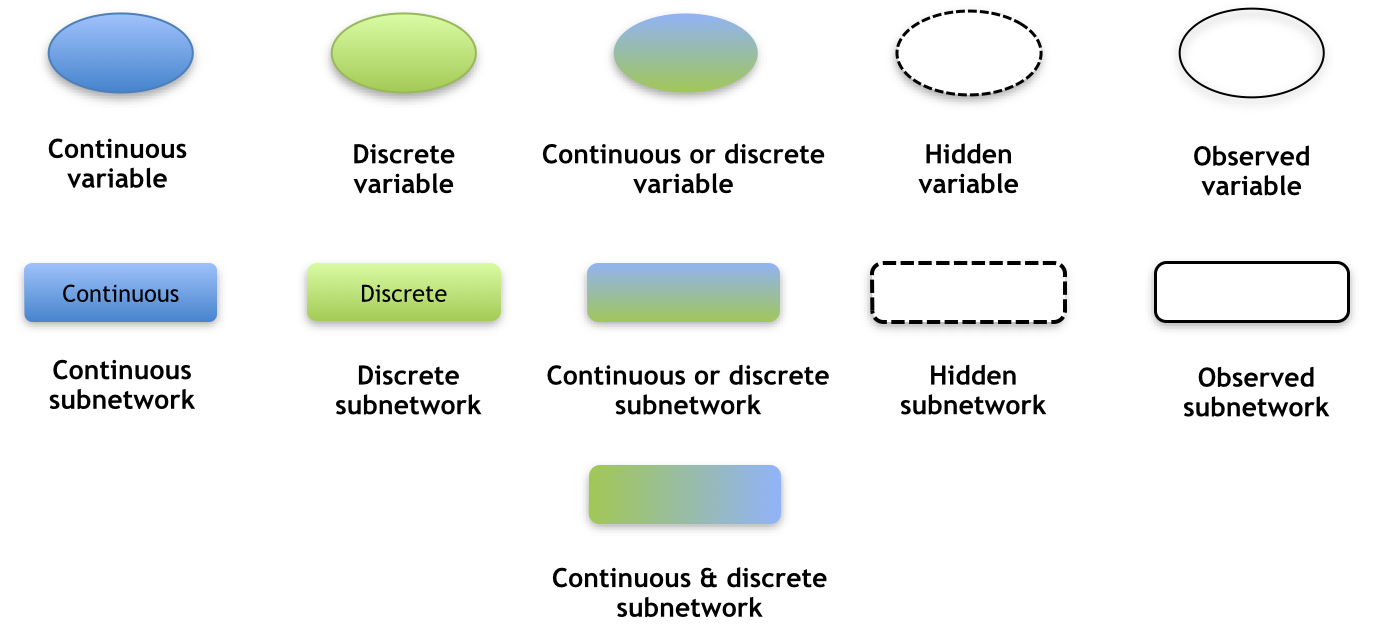
\includegraphics[scale=0.4]{./figures/PreliminariesNotation}
\caption{\label{Figure:PreliminariesNotation}PreliminariesNotation
}
\end{center}
\end{figure}

For regular types of dynamic Bayesian networks we usually assume that observations are made at a fixed frequency. The interval between time slices vary from problem to problem, and we will use the notation $\bm X_{a:b}$ to denote the set of variables from $\bm X_a$ to $\bm X_b$. We need to specify how the world evolves (the transition model) and how the observed variables get their values (sensor model). The transition model specifies the probability distribution of the state variables at $t$ given the previous values, that is, $P(X_t|\bm X_{0:t-1})$. As $t$ increases the set $X_{0:t-1}$ becomes intractable. To reduce the number of links we resort to the well-known Markov assumption, for which the current state is independent from the past given a finite number of previous steps. In particular, we will consider a \textbf{first-order Markov chain} and assume that knowing the present makes the future conditional independent from the past, that is, : $P(\bm X_t|\bm X_{0:t-1}) = P(\bm X_t|\bm X_{t-1})$ (see Figure \ref{Figure:markovChain}).

\begin{figure}
\begin{center}
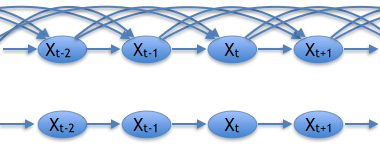
\includegraphics[scale=0.56]{./figures/PreliminariesMarkovChain}
\caption{\label{Figure:markovChain}DBN assuming a third-order Markov property (above) and a first-order Markov property (below).
}
\end{center}
\end{figure}

In order to increase the accuracy of the approximation of using a first-order Markov model, we could either increase the Markov order or equivalently, increase the number of state variables, which would also increase the complexity. Hence, we would like to come up with models that contain a self-sufficient set of variables, which likewise requires to fully understand the ``physics''  of the process being modelled for the different use cases \cite{russelNorvig2009}. 


We still face the problem of having to specify a different distribution for each time slice. To avoid this problem, we assume that changes in the world state are driven by a \textbf{stationary process}, that is, $P(\bm X_{t+1}|\bm X_{t} =\bm X_t|\bm X_{t-1})\ \forall t$.



In the following sections we present the simplest instantiations of a DBN, such as Hidden Markov models and Kalman filters.

\subsubsection*{Hidden Markov models}
A Hidden Markov model (HMM) is the simplest DBN with both hidden and observed variables, in which the state of the process is represented by a single discrete variable. This discrete state variable, which can be in reality the combination of several discrete variables, represents the different possible states of the target problem. Figure \ref{Figure:HMM} shows a graphical example of an HMM\footnote{Although the observed variables are represented as discrete, they can be a combination of discrete and continuous variables}. The advantage of having a single state variable is that all the computations reduce to simple matrix-vector operations .

\begin{figure}
\begin{center}
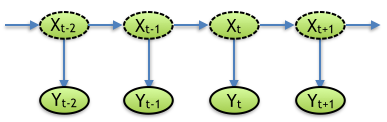
\includegraphics[scale=0.56]{./figures/PreliminariesHMM}
\caption{\label{Figure:HMM}Bayesian network structure corresponding to a HMM.}
\end{center}
\end{figure}

We will represent the sensor (or observation) model by $P(\bm Y_t|\bm X_t)$. Most of our models, although not all of them (Cajamar will be an exception, as shown in Section \ref{Section:CajaMarModels}), will assume that the current state is sufficient to generate the current sensor values. This is referred to as the \textbf{sensor Markov assumption}, that is, $P(\bm Y_t|\bm X_{0:t}, \bm Y_{0:t-1}) = P(\bm Y_t|\bm X_t)$.

By considering the prior probability distribution at time $0$, $P(0)$, we can specify the complete joint distribution over all the variables for any $t$ as:

\begin{equation}
P(\bm X_{0:t},\bm Y_{1:t}) = P(\bm X_0) \prod_{i=1}^t{P(\bm X_i| \bm X_{i-1})P(\bm Y_i|\bm X_i)}
\end{equation}

Although most of our models will fit into this description of observed and hidden (state) variables, there will be cases in which the transition model takes place in observed variables (the case of Cajamar), which in general simplifies the learning-inference processes of the problem.



\subsubsection*{Kalman filters}
Similar to the extension of the static Bayesian network model to hybrid domains, dynamic Bayesian network models have likewise been extended to continuous and hybrid domains. In purely continuous domains, where the continuous variables follow linear Gaussian distributions, the DBN corresponds to (a factorized version of) a Kalman filter (KF). The structure of a KF is exactly the same as the one displayed in Figure \ref{Figure:HMM} for the HMM, although all variables should be considered as continuous. In this case, the state variables can be a combination of continuous variables with different (linear) dependences. In these types of models, the dynamics of the process are assumed to be linear. When modelling non-linear domains, the dynamics and observational distributions are often approximated through, e.g., the extended Kalman filter, which model the system as \textit{locally} linear in the mean of the current state distribution. 

In order to make non-linear prediction we need a more expressive model, such as the \textbf{switching Kalman filter} (SKF). The SKF includes an extra discrete state variable to the network that allows running multiple KFs in parallel. 

\subsubsection*{Dynamic Bayesian networks}

DBN in general can model arbitrary distributions, an example of which can be seen in Figure \ref{Figure:DBN}, where discrete random variables could even have continuous parents. In our models however we will try to remain in the family of the conditional linear Gaussian distributions (CLG), and that is why we will try to avoid discrete children with continuous parents. The probability distributions in the AMIDST models can be parametrized as follows (read notation as parents $\rightarrow$ children):
\begin{itemize}
\item Discrete $\leftrightarrows$ Discrete: distributed as a multinomial distribution conditioned on the discrete parents.
\item Continuous $\leftrightarrows$ Continuous: distributed as (linear) Gaussian/multivariate Gaussian distribution conditioned on the continuous parents (conditional linear Gaussian)
\item Discrete $\rightarrow$ Continuous: distributed as a mixture of Gaussians (the number of components increases exponentially in time if the discrete parent variables are linked through time). 
\end{itemize}


\begin{figure}
\begin{center}
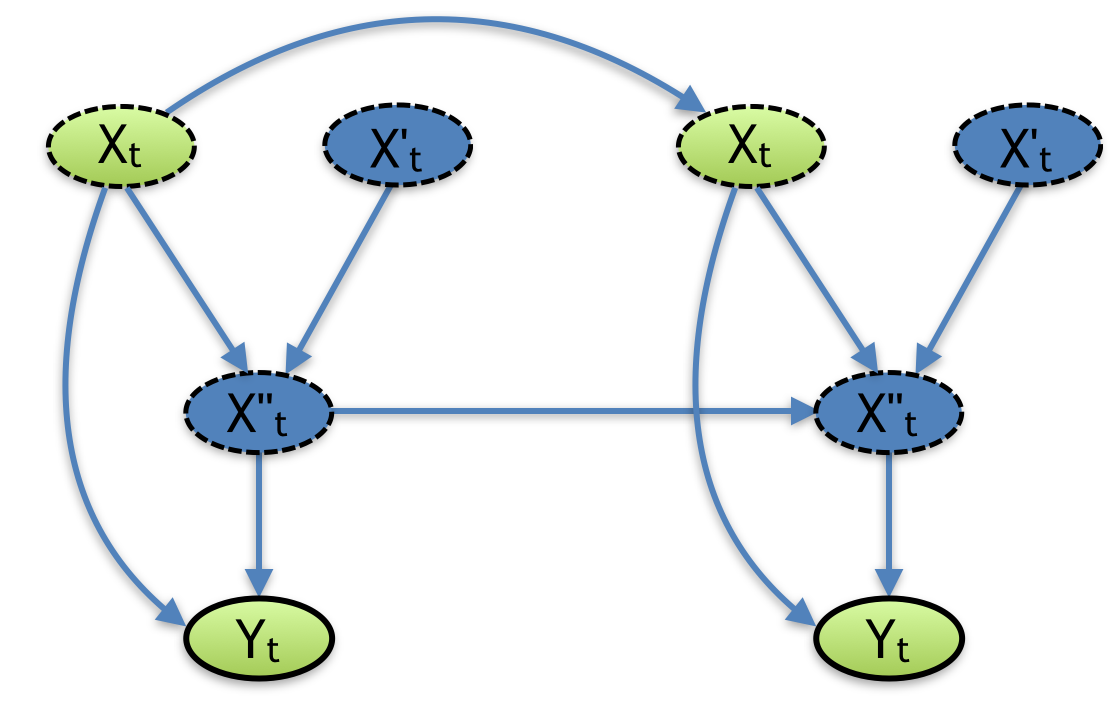
\includegraphics[scale=0.45]{./figures/PreliminariesDBN}
\caption{\label{Figure:DBN}Bayesian network structure corresponding to an example of  unrestricted DBN.}
\end{center}
\end{figure}

The DBN in Figure \ref{Figure:DBN} satisfies the first-order Markov property, and hence can be sufficiently represented by showing two time slices. These restricted DBN are often refereed to as 2-time slice DBN and is usually defined by an initial model representing the initial joint distribution of the process and the transition model (as explained above). 

%- Mention: finite vs infinite horizone?



Note that HMM, KF or SKF are particular cases of DBN. In particular, every HMM can be represented as a DBN with a single state variable and every discrete DBN as a HMM combining all hidden variables into a single state variable. It is however often preferred to factorise the joint distribution taking the structure of the network into account, in order to take advantage of the sparseness in the model. Likewise, every KF can be represented as a DBN with linear Gaussian conditional distributions, but clearly not every continuous DBN can be represented as a KF, sinced the latter is limited to single multivariate Gaussian distributions to model the current state distribution. The advantage of using HMM and KF is that they can benefit from very efficient implementations by using matrix operations.

DBN obviously share the computational difficulties of regular Bayesian networks, but in the dynamic case we are also often faced with the entanglement problem: after a certain time step, all variables describing the current system state will become dependent, and we can therefore not represent the exact probability distribution over the current state (the belief state) in a compact and factorized form. There exist well-known algorithms defined for learning and inference (including most likely explanation). Because of the entanglement problem above mentioned, one often employs approximate methods including approximate factorizations of the joint probability distribution describing the system state \cite{BoyenKoller1998} as well as sampling based techniques in the form of particle filtering \cite{Doucet2000}.

\subsection{Data analysis}\label{SubSection:DataAnalysis}

As already commented in the introduction, the data analysis detailed here will be used to test some assumptions supporting the models elicited by the experts in the different use cases, and also to complement our understanding about the nature of the problem we are modelling. The set of tools employed for this purpose allow us to get insights about some simple and basic aspects of the structural and the distributional assumptions present in a dynamic Bayesian network (DBN).

\subsubsection*{Structural assumptions: sample correlograms and partial correlograms}

A DBN mainly aims to model complex multivariate time series. By using sample correlogramas and sample partial correlograms, we will try to test if the available data supports the temporal correlation between variables assumed by the DBN model, i.e., the temporal links between variables. However, these tools will only allow us to look at univariate time series, what strongly limits the reach of the  extracted conclusions. But, as we will see later in the different use-cases, this analysis will give us some worth insights which could not be elicited from the experts.  

\begin{description}
\item[Sample correlogram:] Let ${x_1,...,x_T}$ be a univariate time series. The \emph{sample autocorrelation coefficient} at lag $v$ is given by 

$$ \hat{\rho}_v =\frac{\sum_{t=1}^{T-v} (x_t-\bar{x})(x_{t+v}-\bar{x})}{\sum_{t=1}^{n} (x_t-\bar{x})^2}$$ 

\noindent where $\bar{x}$ is the sample mean. The plot of $\hat{p}_v$ versus $v$ for $v=1,..., M$ for some maximum $M$ is called the \emph{sample correlogram} of the data. $\hat{p}_v$ corresponds to the Pearson correlation between the series $\{x_t\}_{t\in\{1,...,T\}}$ and $\{x_{t+v}\}_{t+v\in\{1,...,T\}}$.

\item[Sample partial correlogram:] Let us denote by $X_t$ to the random variable associated to $X$ taking values at time $t$. We can build the following regression problem:

$$ X_t = a_0 + a_1X_{t-1} + a_2X_{t-2} + ... a_{v-1}X_{t-v-1}$$

In addition, let $e_{t,v}$ denotes the residuals of this regression problem (i.e., the error when estimating $X_t$ using a linear combination of $v-1$ previous observations). The \emph{sample partial autocorrelation coefficient} of lag $v$, denoted as  $\hat{\theta}_v$, is the standard sample autocorrelation between  the series $\{x_{t-v}\}_{t-v\in\{1,...,T\}}$ and $\{e_{t,v}\}_{t\in\{1,...,T\}}$. Intuitively, the sample partial autocorrelation coefficient of lag $v$ can be seen as the correlation between $X_t$ and $X_{t+v}$ after having removed the common \emph{linear} effect of the data in between.
\end{description}

Sample correlograms can be interpreted as a way to measure the strength of the following unconditional dependences: $X_t  \not\perp X_{t+v}$ for some lag $v \geq 1$.  When $\hat{\rho}_v$ is close to zero, this strongly indicates that there is an unconditional independence between $X_t$ and $X_{t+v}$. However, when $\hat{\rho}_v$ is close to either $1$ or $-1$, this strongly indicates that there is a correlation or dependency between $X_t$ and $X_{t+v}$. But, again, we should never forget that when computing these Pearson correlation coefficients we are making a strong assumption about the normality of the data, which might not hold in the data.

Figure \ref{Figure:PreliminariesCorrelograms} shows an example of how a sample correlogram looks like for two kind of data set: a sequence of 50 data samples i.i.d. according to a Gaussian distribution with zero mean and unit variance $x_t\sim N(0,1)$ (see Figure \ref{Figure:PreliminariesCorrelograms}(a));  and, on the other hand, a sequence of 50 data samples distrubuted as $x_t=x_{t-1} + \epsilon$, such that $\epsilon\sim N(0,1)$ (see  Figure \ref{Figure:PreliminariesCorrelograms}(b)). As can be seen, for the i.i.d. data the correlogram has always values close to zero for all the lags. However, for the time series data, the correlogram clearly identifies the presence of a temporal relationship in the data. As expected, the correlation decreases with the size of the lag, and how quickly it decreases depends on the strength of the temporal relationship. 

Similarly, we plot in Figure \ref{Figure:PreliminariesCorrelograms}(c) and  in  Figure \ref{Figure:PreliminariesCorrelograms}(d) the sample partial correlograms for the same two data sequences presented above. In the case of i.i.d. data, we can see again that the partial correlogram does not show any sign of partial correlation between the data sequence samples. However, for time series data, the partial correlogram takes a high value for $v=1$ (i..e for this lag it is equal to the sample correlogram) and then is null for $v$ higher than 1. Sample partial correlogram can be interpreted as a way to measure the strength of the following conditional dependence: $X_t  \not\perp X_{t+v} | X_1,...,X_{t+v-1}$ for some lag $v>1$.  Accordingly, the sample partial correlogram correctly identifies that we have the following conditional independencies: $X_t\perp X_{t+2}|X_{t+1}$ in this time series data. Therefore, sample partial correlogram can be seen as a tool to test the order of the Markov chain generating a time data sequence, with all the same caveats expressed for the sample correlogram. 

\begin{figure}
\begin{center}
\begin{tabular}{cc}
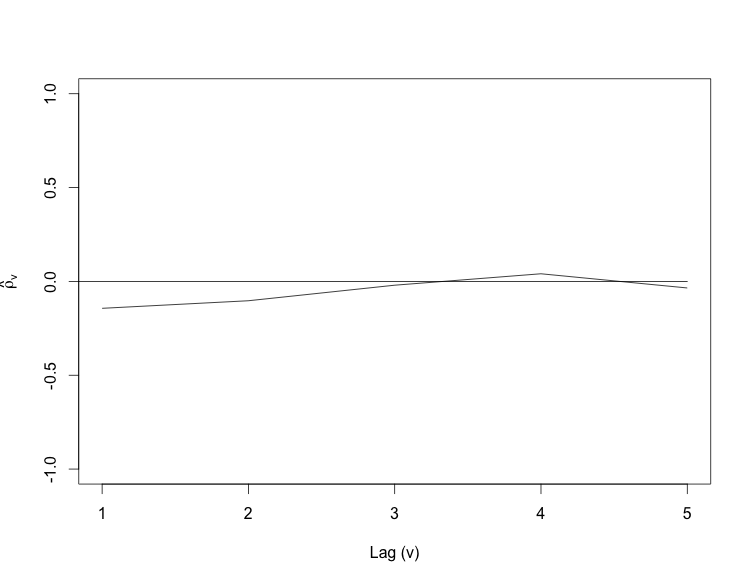
\includegraphics[scale=0.25]{./figures/CorrelogramGaussian} &
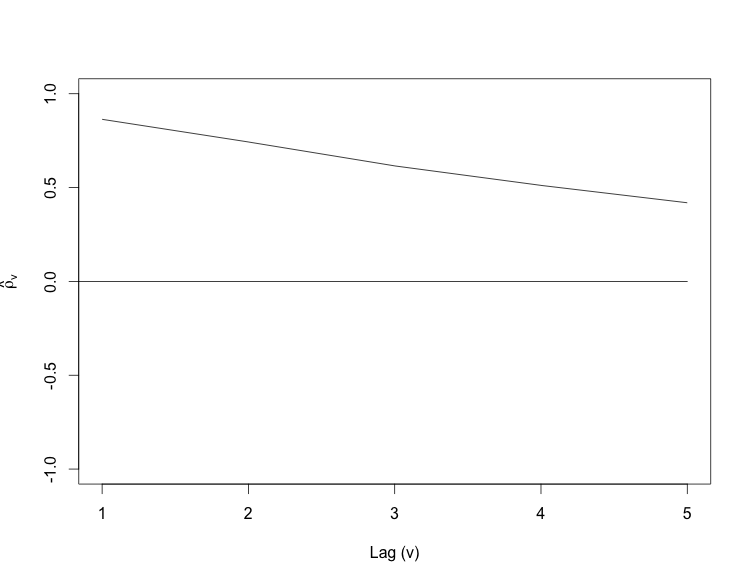
\includegraphics[scale=0.25]{./figures/CorrelogramTimeSerie} \\
(a) Correlogram for i.i.d. data & (b) Correlogram for a time series data \\
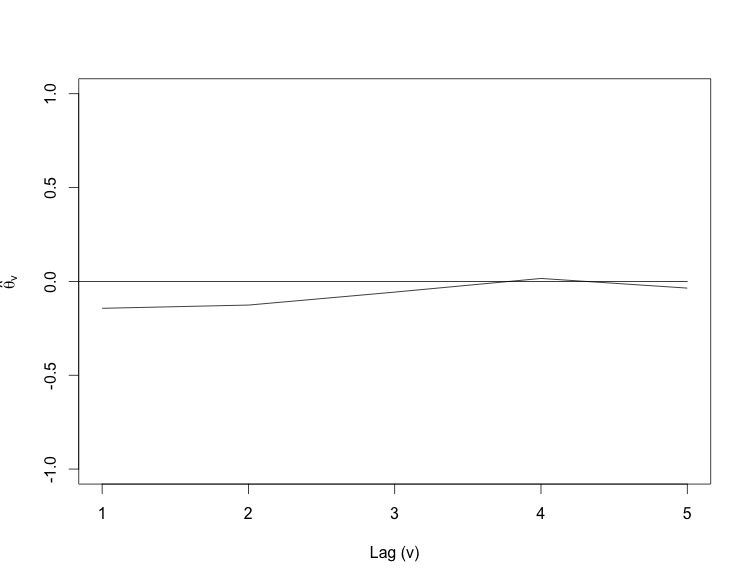
\includegraphics[scale=0.25]{./figures/PartialCorrelogramGaussian} &
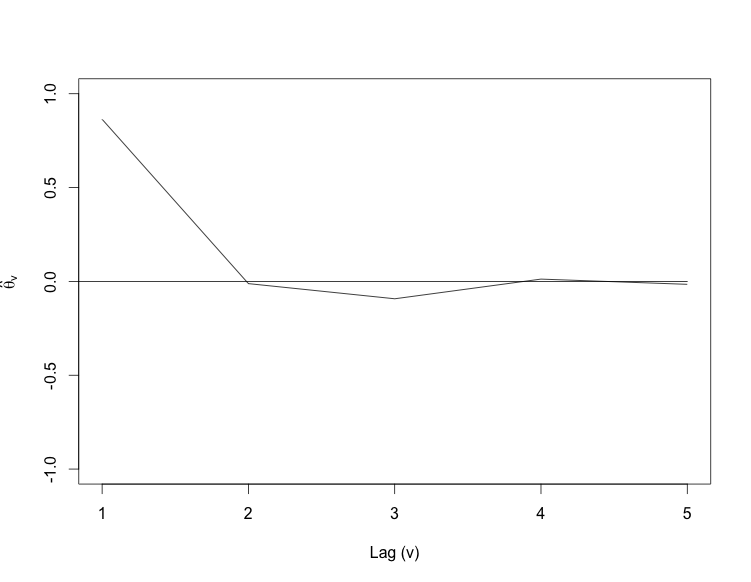
\includegraphics[scale=0.25]{./figures/PartialCorrelogramTimeSerie} \\
(c) Partial correlogram for i.i.d. data & (d) Partial correlogram for a time series data \\
\end{tabular}
\caption{\label{Figure:PreliminariesCorrelograms} Examples of sample correlograms and sample partial correlograms for i.i.d. and time series data. 
}
\end{center}
\end{figure}

\subsubsection*{Distributional assumptions: Histograms and Bivariate Distributions}

With the tools described in this new section we tried now to get insights about the conditional probability distributions of the proposed models. The first basic tool that we employed for this purpose was the histograms. However this tool, although quite useful in a static context, is quite limited in dynamic models. For example, let us assume we have a time series $x_1,\ldots, x_T$ and our histogram shows that the empirical distribution of the variable when we aggregate the data samples over time looks like a mixture of Gaussian distributions. There are two simple possibilities that can give rise to this finding: i)  $X_t$ is distributed according to a mixture of Gaussians where each Gaussian component depends on $X_{t-1}$; ii) there is a discrete hidden variable $Z_t$ that influences $X_{t}$ but which is not observed and it is the one that generates the different mixture components.  As shown in this example, histograms are difficult to interpret in dynamic models, but we will use them when we think that they can be of some help. 

The other tool that we are going to use to get insights about the conditional distributions of the model is the contour plot of the empirical bivariate distribution of $X_t$ versus $X_{t-1}$.  These contour plots can show many relevant information such as if there are linear relationships between variables or if we can assume they are normality distributed, etc. In Figure \ref{Figure:PreliminariesBivariates}, we plot the bivariate contour plot for the i.i.d data and the time series data previously employed when describing the sample correlograms. As can be seen, the bivariate contour plot shows how $X_t$ and $X_{t+1}$ seems to be distributed according to a bivariate normal with a covariance matrix that displays a strong degree of correlation. In the case of i.i.d. data, the contour plot does not reveal  any temporal dependence between $X_t$ and $X_{t-1}$. 

\begin{figure}
\begin{center}
\begin{tabular}{cc}
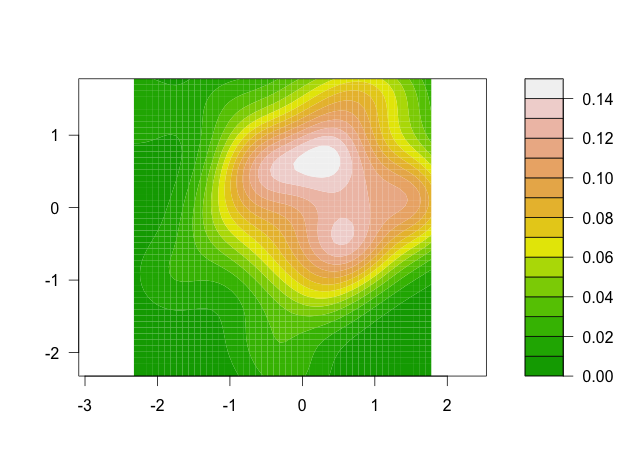
\includegraphics[scale=0.25]{./figures/BivariateGaussian} &
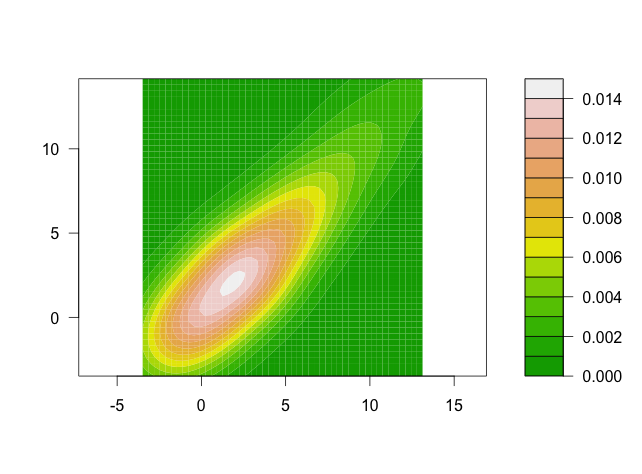
\includegraphics[scale=0.25]{./figures/BivariateTimeSerie} \\
(a) i.i.d. data & (b)  Time series data \\
\end{tabular}
\caption{\label{Figure:PreliminariesBivariates}Bivariate contour plots for a set of i.i.d. data and for a time series data. 
}
\end{center}
\end{figure}
